Los \'oxidos mixtos est\'an formados por dos o m\'as cationes met\'alicos y ox\'igeno. Ellos forman una gran  familia de compuestos que presenta diferentes estructuras, propiedades y funcionalidades. Entre los tipos de estructuras las perovskitas son importantes debido a su gran variedad de propiedades y composiciones cuya formula general es $ABO_{3}$. El nombre perovskita fue tomado de un mineral hom\'onimo con dicha estructura ($CaTiO_{3}$) descubierto en 1839 en los montes Urales por Gustav Rose y se le nombr\'o en honor al mineralogista ruso Lev Alexeievitch Perovski.


\noindent Las perovskitas presentan estructuras de tipo tetragonal, ortorr\'ombica o rombo\'edrica las cuales son distorsiones de una estructura con simetr\'ia cubica. Adem\'as presentan propiedades que dependen de factores como la temperatura, composici\'on qu\'imica, presi\'on y campo el\'ectrico. Estas propiedades tienen aplicaci\'on en la fabricaci\'on de sensores, transductores, osciladores, dispositivos de almacenamiento de informaci\'on entre otras.


\noindent Los materiales multiferroicos fueron descubiertos el siglo pasado \cite{wang2003}, pero no fueron estudiados debido a que la f\'isica de la materia condensada en ese momento consideraba al magnetismo y a la ferroelectricidad como propiedades mutuamente excluyentes. El inter\'es en estos materiales resurgi\'o a inicios del siglo XXI en el a\~no 2003 con el trabajo de Spaldin y sus colaboradores \cite{spaldin2005}. En este trabajo se present\'o una hip\'otesis para la poca cantidad de ferroel\'ectricos magn\'eticos y adem\'as se analizaron las t\'ecnicas m\'as modernas de s\'intesis y caracterizaci\'on de estos materiales. En la figura \ref{EstadisticaPublicaciones} se puede observar la cantidad de art\'iculos cient\'ificos relacionados con el t\'ermino {\bf multiferroic} en algunas bases de datos, de las m\'as importantes en ciencia de materiales y/o f\'isica, donde se aprecia que la cantidad ha aumentado en el periodo 2003 - 2013 mostrando el inter\'es en estudiar este tipo de materiales.


% -------------------------------------
% FIGURA: estadistica de publicaciones
% -------------------------------------

\begin{figure}[H]
\centering
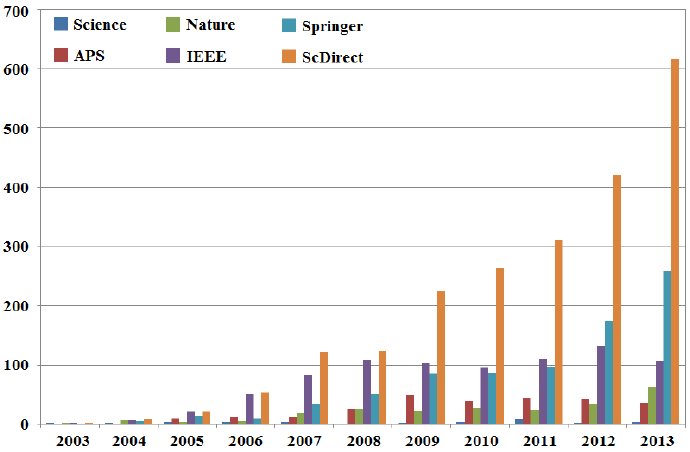
\includegraphics[width=0.9\textwidth]{contenido/introduccion/img_introduccion/EstadisticaPublicaciones.png}
\caption[Estad\'istica de publicaciones]{N\'umero de publicaciones anuales 
2003 - 2013 
en las bases de datos: Science, American Physical Society, Nature, IEEE, 
Springer, ScienceDirect}
\label{EstadisticaPublicaciones}
\end{figure}

\noindent El nombre multiferroico se le otorga a los materiales que poseen en una misma fase cristalina dos o m\'as ordenes ferroicos primarios tales como: ferroelasticidad, ferroelectricidad, ferromagnetismo o ferrotoroicidad. Tambi\'en es posible considerar ordenes  antiferroicos. En su mayor\'ia los materiales ferroel\'ectricos y espec\'ificamente las perovskitas presentan propiedades ferroel\'asticas provocadas por la asociaci\'on entre la deformaci\'on de la estructura cristalina y la polarizaci\'on. Desde un punto de vista pr\'actico, los materiales multiferroicos que atraen mayor inter\'es presentan acoplamiento entre ferroelectricidad y magnetismo. Estos materiales son denominados multiferroicos magnetoel\'ectricos debido a que un campo el\'ectrico puede cambiar la polarizaci\'on y la magnetizaci\'on, tambi\'en es posible que un campo magn\'etico cambie la polarizaci\'on.

\noindent La ferrita de bismuto ($BiFeO_{3}$) es una perovskita bastante estudiada entre los materiales multiferroicos debido a que presenta un acoplamiento magnetoel\'ectrico y orden multiferroico a temperatura ambiente acompa\~nado de una estructura cristalina simple. Smolensky y sus colaboradores fueron los primeros en estudiar la ferrita de bismuto en 1959 pero sus muestras resultaron ser muy conductivas para dar resultados adecuados. Este material atrajo inter\'es a partir de los resultados presentados por Wang y sus colaboradores \cite{wang2003}, estos resultados mostraban una gran polarizaci\'on remanente {\bf P} la cual era quince veces mayor a observaciones previas junto con un gran ferromagnetismo de $1.0 \mu _{B}$ por celda unitaria. Pero algunos resultados fueron luego encontrados err\'oneos. A pesar de ello el trabajo inspir\'o un gran n\'umero de estudios experimentales y te\'oricos de este material. A pesar de haber sido muy estudiada la ferrita de bismuto, en la actualidad se siguen descubriendo nuevas caracter\'isticas de este material. Por ejemplo, se siguen descubriendo nuevas fases cristalinas en funci\'on de la temperatura y/o la presi\'on \cite{teague1970,koumpouras2011}, por lo que su diagrama de fases a\'un es desconocido en su totalidad. Tambi\'en se pueden hallar nuevas propiedades como el aumento de la conductividad en algunos dominios espec\'ificos \cite{ravindram2006} o propiedades de respuesta bastante \'utiles en pel\'iculas delgadas \cite{spaldin2005}.


\noindent El caso de la cromita de itrio ($YCrO_{3}$) es algo diferente ya que este material fue reconocido como multiferroico recientemente, siendo clasificado como un material biferroico perteneciente al grupo de cromitas de tierras raras. Como un material multiferroico comparte las mismas posibles aplicaciones que la ferrita de bismuto.


\noindent El objetivo del presente trabajo es el estudio de la estructura 
electr\'onica de la ferrita de bismuto ($BiFeO_{3}$) y de la cromita de itrio ($YCrO_{3}$), para ello se calcul\'o la densidad de estados
electr\'onicos, el diagrama de bandas de energ\'ia y la densidad de carga. Para 
ello se utilizaron los arreglos antiferromagn\'eticos tipo A y G para la ferrita de bismuto y los arreglos antiferromagn\'eticos tipo A, C y G para la cromita de itrio, con el fin de observar su comportamiento y determinar cual seria el m\'as estable entre ellos.Lo anterior ser\'a realizado mediante el uso de la teor\'ia del funcional de densidad; implementada en el paquete de simulaci\'on Quantum ESPRESSO. Adem\'as se utilizara pseudopotenciales ultrasuaves junto a la aproximaci\'on de densidad local considerando adem\'as el par\'ametro de Hubbard con un valor de $2.43$ eV y $1.13$ eV para los \'atomos de hierro y cromo respectivamente.
